%%%%%%%%%%%%%%%%%%%%%%%%%%%%%%%%%%%%%%%%%
% Szablon pracy dyplomowej
% Wydział Informatyki 
% Zachodniopomorski Uniwersytet Technologiczny w Szczecinie
% autor Joanna Kołodziejczyk (jkolodziejczyk@zut.edu.pl)
% Bardzo wczesnym pierwowzorem szablonu był
% The Legrand Orange Book
% Version 5.0 (29/05/2025)
%
% Modifications to LOB assigned by %JK
%%%%%%%%%%%%%%%%%%%%%%%%%%%%%%%%%%%%%%%%%


%----------------------------------------------------------------------------------------
%	CHAPTER 2
%----------------------------------------------------------------------------------------
\sloppy

\chapter{Opis architektury systemu}

W tym rozdziale zostaną szczegółowo przedstawione kwestie związane z architekturą aplikacji do udostępniania materiałów edukacyjnych. Omówiona zostanie architektura aplikacji, struktura bazy danych Hazelcast, podział aplikacji na moduły, najważniejsze aspekty związane z realizacją konkretnych funkcjonalności i przedstawione zostaną diagramy klas, przypadkow użycia, komponentów i związków encji

\section{Architektura aplikacji}

Aplikacja została oparta o wzorzec architektoniczny MVC (\textit{Model-View-Controller}), który zapewnia czytelny podział aplikacji na warstwy:

\begin{itemize}
\item \textbf{Model} – reprezentujący logikę biznesową oraz struktury danych. Realizowany jest za pomocą klas encji oraz repozytoriów Spring Data.
\item \textbf{View} – odpowiedzialny za prezentację danych użytkownikom końcowym. Do jego realizacji wykorzystano szablony Thymeleaf oraz biblioteki Bootstrap.
\item \textbf{Controller} – obsługujący żądania użytkowników oraz zapewniający komunikację pomiędzy widokiem a modelem aplikacji.
\end{itemize}

Takie podejście zapewnia przejrzystą strukturę projektu, ułatwiając jego dalszą rozbudowę oraz utrzymanie \cite{microservices}.

\section{Wymagania funkcjonalne aplikacji}
\begin{itemize}
\item Aplikacja umożliwi użytkownikom rejestrację konta przy użyciu unikalnej nazwy użytkownika, hasła i adresu e-mail, aplikacja będzie walidować czy nazwa użytkownika i mail nie są już wykorzystane przez innego użytkownika.
\item 
Aplikacja umożliwi logowanie i będzie prowadziła kontrolę dostępu opartą na rolach, rozróżniając role administrator, nauczyciel i użytkownik w celu ograniczenia lub przyznania dostępu do określonych stron i działań.
\item Administratorzy będą mogli tworzyć, edytować i usuwać lekcje i kursy, przypisywać nauczyciela do dowolnych kursów
\item Administratorzy będą mogli zarządzać wszystkimi profilami użytkowników, dodawać, usuwać użytkowników.
\item Administratorzy Będą mogli publikować materiały edukacyjne, kursy i lekcje
\item 
Nauczyciele będą mogli tworzyć, aktualizować i usuwać lekcje w ramach przypisanych im kursów oraz dodawać zadania do lekcji które opcjonalnie będą miały date do kiedy można rozwiązanie przesłać.
\item 
Użytkownicy będą mogli zapisywać się na dostępne zajęcia, następnie po zapisaniu się na kurs będą mogli przeglądać dostępne lekcje w danym kursie.
\item Użytkownicy będą mogli przesyłać rozwiązania do zadań stworzonych przez nauczycieli bądz Administratora.
\item Aplikacja powinna umożliwić nauczycielą i Administratorą ocenę przesłanych rozwiązań przez użytkowników
\item Aplikacja powinna pokazywać ile czasu zostało do przesłania rozwiązania, oraz czy rozwiązanie jest przesłane po czasie
\item Nauczyciele i Administratorzy powinni móc dodawać materiały edukacyjne, dostępne dla każdego.
\item Aplikacja powinna umożliwić dodawanie komentarzy, polubień i ocenienia materiału dodanego przez Administratora bądz nauczyciela.
\item Aplikacja powinna umożliwić dodanie tylko jednego polubienia i oceny jednemu użytkownikowi pod danym materiałem.
\item Aplikacja powinna trzymać statystyki w panelu administratora
\item Aplikacja powinna implementować sesje HTTP wspierane przez Hazelcast, z limitami czasu bezczynności i ustawianiem plików cookies w celu ochrony sesji użytkowników
\item Aplikacja powinna zawierać panel użytkownika, gdzie użytkownik może zmienić nazwisko, imię i email oraz może sprawdzić do których kursów jest zapisany i czy musi przesłać rozwiązanie do lekcji w którymś z tych kursów
\item Aplikacja powinna zawierać panel nauczyciela, gdzie użytkownik z rolą nauczyciela może zarządzać kursami do których jest przypisany oraz oceniać przesłane rozwiązania przez użytkowników.

\end{itemize}

\section{Struktura bazy danych Hazelcast}

Aplikacja wykorzystuje bazę danych Hazelcast działającą w pamięci operacyjnej. Wszystkie dane aplikacji przechowywane są w mapach Hazelcast, w tym:

\begin{itemize}
\item \textbf{users} – przechowuje dane użytkowników aplikacji, takie jak nazwa użytkownika, hasło, email oraz role.
\item \textbf{posts} – zawiera publikowane materiały edukacyjne wraz z ich szczegółami (tytuł, treść, autor oraz metadane).
\item \textbf{comments} – przechowuje komentarze użytkowników dotyczące materiałów.
 \item \textbf{task\_submissions} -- przechowuje zadania przesłane przez użytkowników oraz ich oceny przez nauczycieli.
  \item \textbf{comment\_likes} -- przechowuje informacje o polubieniach komentarzy.
  \item \textbf{post\_ratings} -- przechowuje oceny materiałów pozostawione przez użytkowników.
  \item \textbf{school\_classes} -- przechowuje informacje o klasach dostępnych dla użytkowników.
  \item \textbf{lessons} -- przechowuje dostępne lekcje przypisane do klas.
  \item \textbf{lesson\_ratings} -- przechowuje oceny lekcji.
  \item \textbf{lesson\_tasks} -- przechowuje zadania przypisane do lekcji przez nauczycieli.
  \item \textbf{app\_statistics} -- przechowuje dane statystyczne aplikacji.
  \end{itemize}

Zastosowanie Hazelcast zapewnia wydajność, skalowalność oraz wysoką dostępność danych \cite{microservices}.

\section{Organizacja kodu źródłowego}

Kod źródłowy aplikacji został zorganizowany zgodnie z zasadami modularności oraz dobrymi praktykami programistycznymi. Struktura projektu dzieli się na moduły:

\begin{itemize}
\item \textbf{Moduł \texttt{persistent}} – odpowiedzialny za zarządzanie danymi aplikacji przechowywanymi w Hazelcast.
\item \textbf{Warstwa usług (\textit{Services})} – udostępniająca logikę biznesową oraz operacje na danych.
\item \textbf{Warstwa kontrolerów} – odpowiada za obsługę żądań HTTP oraz zarządzanie widokami.
\item \textbf{Warstwa widoków (Thymeleaf)} – odpowiedzialna za generowanie dynamicznych stron HTML.
\end{itemize}

\section{Implementacja najważniejszych funkcjonalności}

Do kluczowych funkcjonalności systemu, których implementacja została omówiona w tej pracy należą:

\begin{itemize}
\item \textbf{System uwierzytelniania i autoryzacji} – oparty o Spring Security, umożliwiający zarządzanie dostępem do zasobów aplikacji zgodnie z rolą użytkowników.
\item \textbf{Publikacja i zarządzanie materiałami edukacyjnymi} – umożliwia użytkownikom tworzenie, edytowanie i usuwanie materiałów.
\item \textbf{Komentowanie i ocenianie materiałów} – pozwala na interakcję użytkowników oraz ocenianie publikowanych materiałów edukacyjnych.
\item \textbf{System statystyk i analiz} – regularnie aktualizowany przez zaplanowane zadania (\textit{Scheduler}), umożliwiający analizę aktywności użytkowników oraz popularności materiałów.
\end{itemize}

Każda z tych funkcjonalności została dokładniej omówiona wraz z przykładami kodu źródłowego ilustrującymi kluczowe elementy implementacji.

\section{Diagramy UML i przypadki użycia}

Dla przejrzystego przedstawienia architektury aplikacji oraz interakcji użytkowników z systemem, zostały przygotowane następujące diagramy UML:

\begin{figure}[H] % Try to place it exactly here
    \centering % Center the figure
    % Use the PDF generated from SVG for best quality
    \includegraphics[width=\linewidth]{Dyplom-styl/svg-32.pdf} % Make sure this filename is correct and it's a PDF
    \caption{Diagram klas, Źródło: opracowanie własne}
    \label{fig:system_klas_zadan}
\end{figure}
Diagram skupia się wyłącznie na klasach domenowych i ich zależnościach do tych klas należą User, SchoolClass, Lesson, LessonTask, TaskSubmission, Post, Comment, PostRating, CommentLike, ClassSignUp, LessonRating. Na diagramie można zauważyć że użytkownik zapisuje się do klasy przez ClassSignup, lekcja agreguje zadania, a oceny i polubienia są encjami asocjacyjnymi. Przyjęto, że tylko nauczyciel i admin tworzą lekcje, zadania, dodają Posty i oceniają rozwiązania wysłane przez użytkowników, zaś użytkownicy mogą składać rozwiązania wystawiać oceny lekcją i postom i dodają komentarze, co wprost wynika z kierunku asocjacji i ról widocznych na diagramie
\begin{figure}[H]
  \centering
  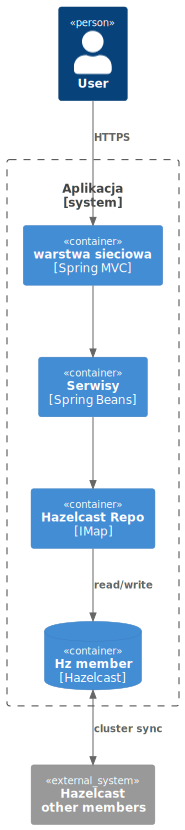
\includegraphics[
        width=\linewidth,
        height=0.8\textheight,   % nie przekrocz 80 % wysokości strony
        keepaspectratio          % zachowaj proporcje
  ]{Dyplom-styl/sv-10.pdf}
  \caption{Diagram komponentów Źródło: opracowanie własne}
  \label{fig:system_klas_zadan}
\end{figure}
diagram pokazuje przepływ: Klient->Web->Serwis->Repo->Hazelcast<->Klaster, użytkownik komunikuje się z systemem przez protokół HTTPS. Warstwe sieciową aplikacji tworzą kontrolery, wykonywana jest tam również walidacja żądań. serwisy tworzą logike domenową, hazelcast repo tworzy warstwe dostępu do danych. Operacje czytania i zapisywania są wykonywane na węźle klastra Hazelcast działającym w aplikacji, natomiast Hazelcast other members pozostałe węzły klastra. Dane są synchronizowane w klastrze.
\begin{figure}[H]
  \centering
  \includegraphics[
        width=\linewidth,
        height=0.8\textheight,   % nie przekrocz 80 % wysokości strony
        keepaspectratio          % zachowaj proporcje
  ]{Dyplom-styl/erd-22.pdf}
  \caption{Diagram ERD Źródło: opracowanie własne}
  \label{fig:system_klas_zadan}
\end{figure}
Diagram pokazuje powiązania pomiędzy tabelami w bazie danych, \begin{itemize}
    \item \texttt{users}: użytkownicy, unikalne pola to \texttt{username} i \texttt{email} zawiera również pola przechowujące imie nazwisko role i hasło.
    \item \texttt{school\_classes}: klasy, z kluczem obcym \texttt{teacher\_id}, który odnosi się do tabeli \texttt{users}.
    \item \texttt{class\_signups}: zapisy do klas, zawiera dwa klucze obce: \texttt{user\_id} oraz \texttt{school\_class\_id}, a także pola statusu i daty.
    \item \texttt{lessons}: lekcja, zawiera \texttt{school\_class\_id}, \texttt{user\_id}, treść, załącznik, termin oddania oraz informację, czy jest dodane zadanie do lekcji.
    \item \texttt{lesson\_tasks}: zadanie przypisane do lekcji (\texttt{lesson\_id}), z terminem i informacją o tym, czy jest wymagane.
    \item \texttt{task\_submissions}: rozwiązania przesłane przez użytkowników (\texttt{lesson\_task\_id}, \texttt{user\_id}), opcjonalny plik bądź tekst, data wysłania, ocena oraz komentarz nauczyciela.
    \item \texttt{lesson\_rating}: oceny lekcji, zawiera dwa klucze obce: \texttt{lesson\_id} i \texttt{user\_id}, oraz pole rating czyli ocenę lekcji.
    \item \texttt{posts}: posty zawierają: autora, treść, ścieżkę załącznika, liczbę wyświetleń oraz średnią ocenę z ocen wystawionych przez użytkowników.
    \item \texttt{comments}: komentarze do postów, z treścią i liczbą polubień.
    \item \texttt{post\_ratings}: oceny postów, z kluczami obcymi \texttt{post\_id} i \texttt{user\_id}, oraz polem rating.
    \item \texttt{comment\_likes}: polubienia komentarzy, zawiera, klucz obcy commentId oraz username.
\end{itemize}
\begin{figure}[H]
  \centering
  \includegraphics[
        width=\linewidth,
        height=0.8\textheight,   % nie przekrocz 80 % wysokości strony
        keepaspectratio          % zachowaj proporcje
  ]{Dyplom-styl/useCase-1-35.pdf}
  \caption{Diagram przypadków użycia -  ogólny zakres funkcjonalności platformy  Źródło: opracowanie własne}
  \label{fig:system_klas_zadan}
\end{figure}
Powyższy diagram przedstawia ogólny zakres funkcjonalności platformy materiałów edukacyjnych, ukazując kluczowe interakcje różnych użytkowników z systemem. Anonimowi użytkownicy mogą przeglądać publiczne materiały oraz rejestrować się i logować do systemu. Zarejestrowani studenci, oprócz przeglądania, mogą wyszukiwać i filtrować materiały, oceniać je i komentować, zapisywać się do klas oraz przesyłać rozwiązania zadań. Nauczyciele mają możliwość przeglądania i wyszukiwania materiałów, ich oceniania i komentowania, a także publikowania i edytowania własnych lekcji i postów oraz oceniania przesłanych zadań. Administratorzy odpowiadają za zarządzanie użytkownikami i statystykami systemowymi, a także mogą rozszerzać swoje działania o publikowanie i edytowanie materiałów.
\begin{figure}[H]
  \centering
  \includegraphics[
        width=\linewidth,
        height=0.8\textheight,   % nie przekrocz 80 % wysokości strony
        keepaspectratio          % zachowaj proporcje
  ]{Dyplom-styl/useCase-2-32.pdf}
  \caption{Diagram przypadków użycia - zarządzanie lekcjami i kursami Źródło: opracowanie własne}
  \label{fig:system_klas_zadan}
\end{figure}
Powyższy diagram koncentruje się na szczegółowym przebiegu interakcji między Nauczycielem a Studentem w kontekście zarządzania klasami, lekcjami i zadaniami. Nauczyciel może tworzyć nowe klasy, publikować lekcje, a następnie tworzyć zadania dla tych lekcji. Ma także uprawnienia do zatwierdzania lub odrzucania próśb o zapisanie się do klasy, przeglądania i oceniania przesłanych rozwiązań zadań, a także generowania statystyk. Student natomiast może prosić o zapisanie się do klasy, przeglądać zawartość lekcji oraz przesyłać rozwiązania zadań. Diagram ilustruje również, jak tworzenie klasy obejmuje publikację lekcji, publikacja lekcji. Zapisanie do klasy pozwala studentowi na przeglądanie zawartości lekcji, ocena zadań aktualizuje statystyki.

\begin{figure}[H]
  \centering
  \includegraphics[
        width=\linewidth,
        height=0.8\textheight,   % nie przekrocz 80 % wysokości strony
        keepaspectratio          % zachowaj proporcje
  ]{Dyplom-styl/useCAse33.pdf}
  \caption{Diagram przypadków użycia -  przesyłanie i ocenianie rozwiązań do zadań  Źródło: opracowanie własne}
  \label{fig:system_klas_zadan}
\end{figure}
Powyższy diagram przedstawia przepływ akcji związanych z zadaniami. Nauczyciel tworzy zadanie do lekcji bedącej częścią klasy(przedmiotu) do którego uczeń(user) należy następnie uczeń przesyła rozwiązanie, nauczyciel wystawia ocene ewentualnie dodaje komentarz i na końcu użytkownik może sprawdzić ocene oraz komentarz dodany przez nauczyciela.